\chapter{Packing shapes on a Plane}

It is known that shape is an important attribute for crystal packings~\tocite, small changes in shape can lead to large changes in the packing fraction and the space group of the resulting crystal. The amorphous packing of shapes has not had the degree of study, focussing on ellipses and circles~\tocite. In this chapter I aim to elucidate the effects that shape has on amorphous packing and how they compare to the crystal packings. Along with generating this database of packing data I will also be looking to identify molecules that are resistant to crystal growth for further study in later chapters. This chapter is concerned with structural elements, exclusively using inherent structures to remove noise from vibrational motion.

The two parameters of the Snowman molecule is the radius and the distance, searching the space of molecules can be done by sampling structures over values of these variables. The ranges of these variables that we chose to search over was
\begin{align}
            r &= [0.5, 1] \\
            d &= [1,1+r]
\end{align}
the range of the radius chosen to display behaviour markedly different to a disc. The distance $d=1$ was chosen as the initial value as previous research~\tocite showed interesting behaviour of crystal packings at that value. The other end of the range corresponds to an equimolar binary disc packing of which there are a number of known \emph{compact packings}~\figref{binary-packings}~\cite{heppes:03,kennedy:06}. One of these optimal packings $r=0.637556$ was included in the survey, it was anticipated that it could show markedly different characteristics than nearby snowmen.

\begin{figure}
    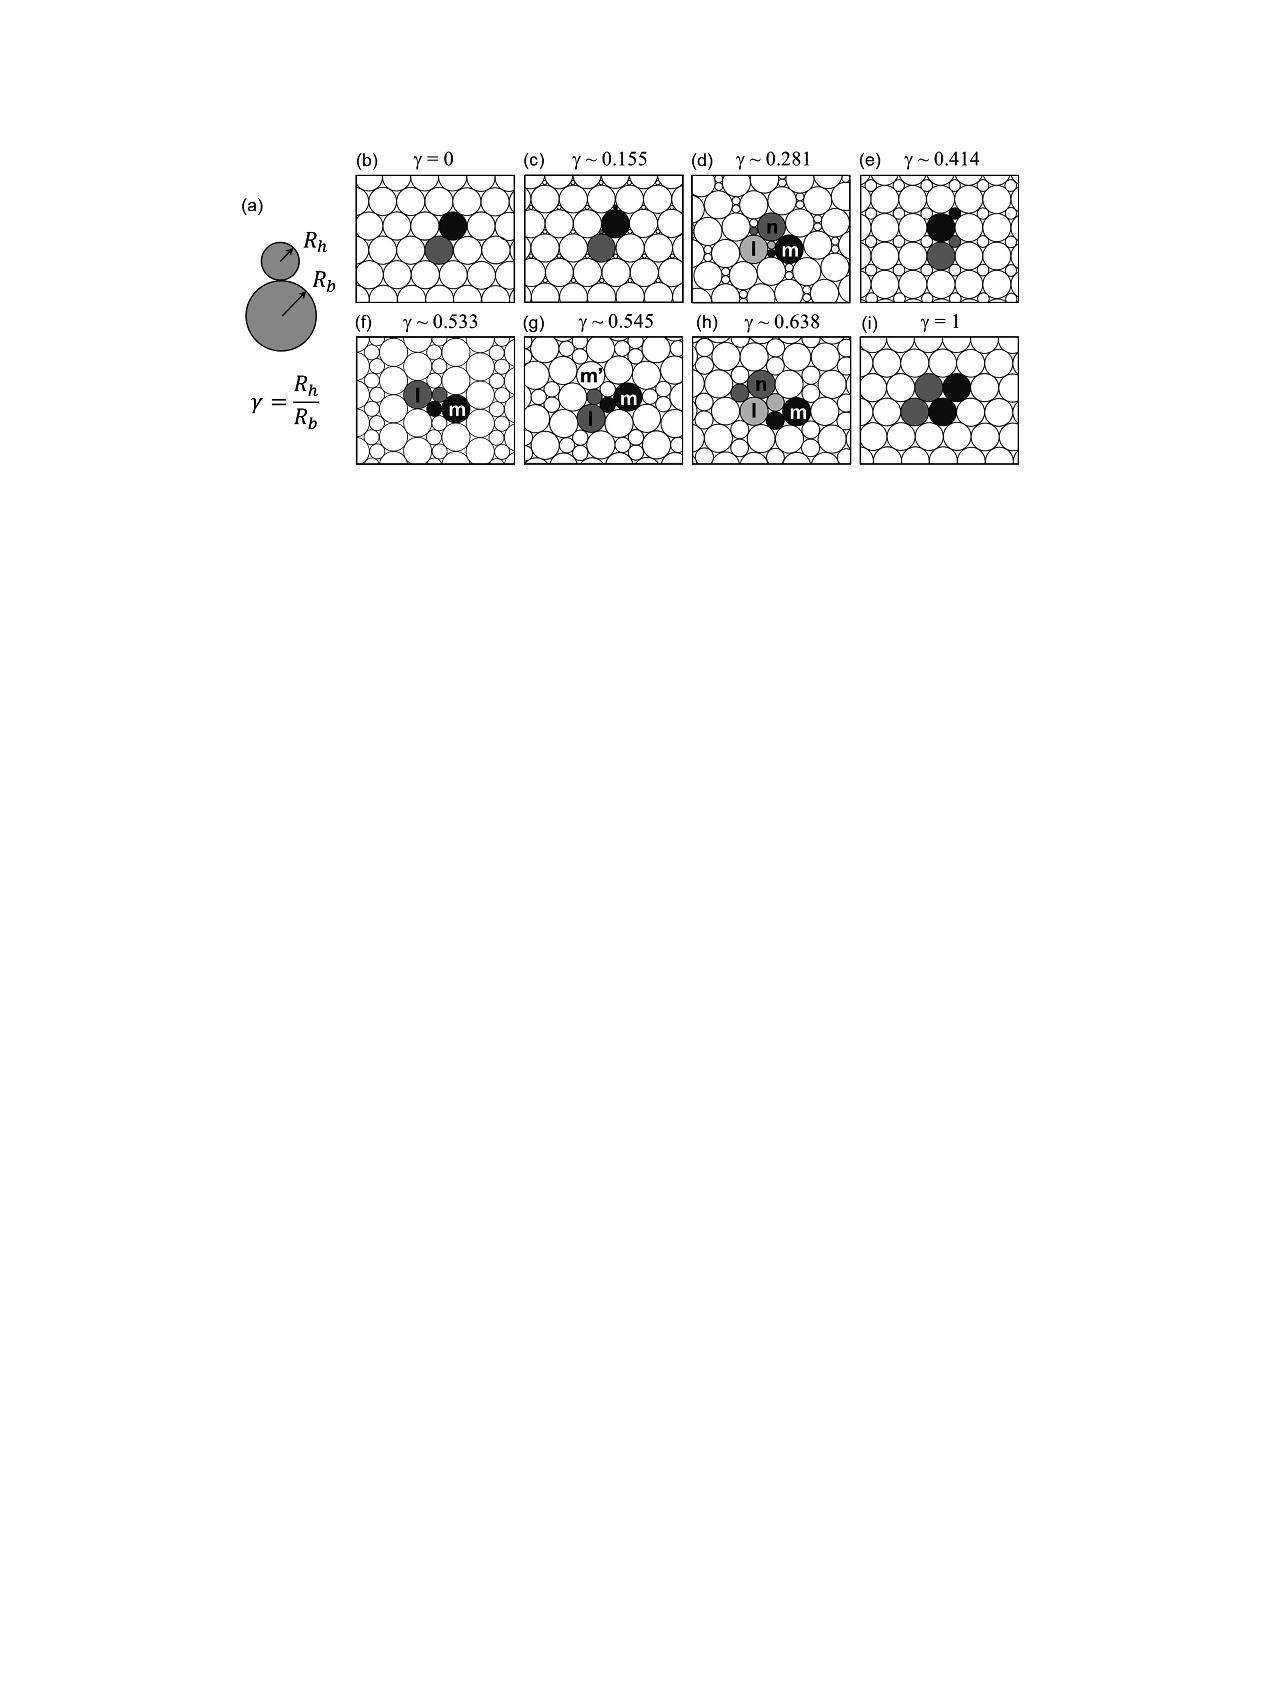
\includegraphics[width=\textwidth]{binary-packings}
    \caption[Perfect binary packings]{The eight perfect equimolar binary packings. All of these are maximums in the packing of space by snowmen crystals.}
    \source{han:13}{American Physical Society}
    \label{fig:binary-packings}
\end{figure}

For trimers the extra dimension makes a complete too computationally expensive. Instead it makes sense to focus on the remaining dimension, the angle, over a range of radii and at both $d=1$ and $d=1+r$.


\section{Packing Dimers}

The packing fraction is a concept used to asses the packing of hard shapes and it can also describe the packing of soft shapes. Taking the inherent structures after equilibration at a temperature of 3.0, the packing fraction of the Snowmen is shown in \textfigref{snowman dist high} and \textfigref{snowman radius high}. As the distance increases from $1$ to $1+r$ the packing fraction drops, this is a result of the overlap of the molecule increasing. At $d=1+r$ the two particles are touching, decreasing the distance results in overlap and a filling of the space between the molecules that was previously unoccupied. The decrease in packing fraction as a function of distance breaks down for four molecules, $d=1+0.8r, 1+r$ and $r=0.9, 1.0$. The cause of this anomaly is not immediately obvious, since our simulations are in two dimensions we can examine the configuration~\figref{snowman 0.9 1.7 frame high}. Here we can see a high degree of order in the packing, while the orientation of the bonds is distributed randomly, the packing is crystalline, as shown by the pair distribution function in~\textfigref{Snowman 0.9 1.7 radial high}. This crystalline order forms in the inherent structure despite the initial state being well above the melting point, a behaviour exhibited by soft discs; the molecule is an excellent crystal former.

\begin{figure}
    \centering
    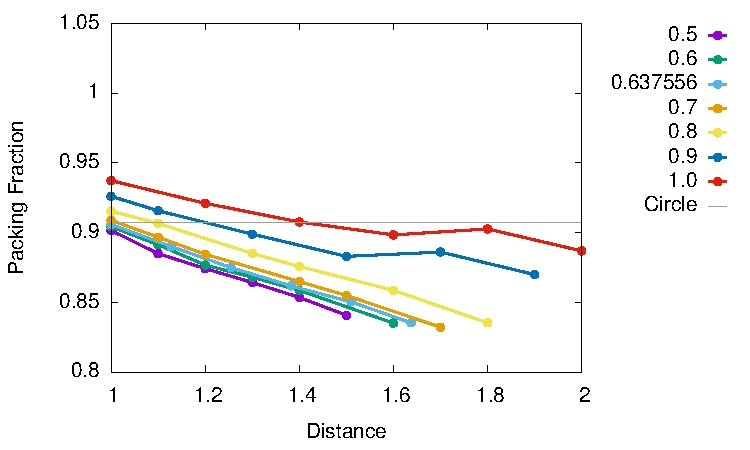
\includegraphics[width=0.75\textwidth]{dist-high}
    \caption[Packing fraction of snowmen as a function of distance ($T=3.0$)]{The packing fraction as a function of distance for the snowman molecules. For reference the optimal circle packing of 0.91 is included.}
    \label{fig:snowman dist high}
\end{figure}

\begin{figure}
    \centering
    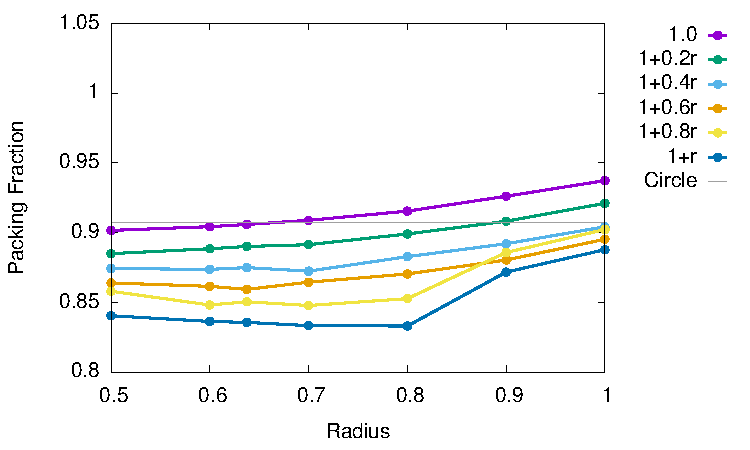
\includegraphics[width=0.75\textwidth]{radius-high}
    \caption[Packing fraction of snowmen as a function of radius ($T=3.0$)]{The packing fraction as a function of radius for the snowman molecules. For reference the optimal circle packing of 0.91 is included.}
    \label{fig:snowman radius high}
\end{figure}

\begin{figure}
    \centering
    \includegraphics[width=\textwidth]{{{Snowman-3.0-0.9-1.7-frame}}}
    \caption[Inherent structure of Snowman $r=0.9$ $d=1.7$]{Inherent structure of the Snowman $r=0.9$ $d=1.7$.}
    \label{fig:snowman 0.9 1.7 frame high}
\end{figure}

\begin{figure}
    \centering
    \includegraphics[width=0.75\textwidth]{{{Snowman-3.0-0.9-1.7-radial}}}
    \caption{Pair distribution function of Snowman with  $r=0.9$ and  $d=1.7$}
    \label{fig:snowman 0.9 1.7 radial high}
\end{figure}

With a number of molecules forming crystalline packings we went looking for crystalline order in the rest of the packings. There are a number of particles with crystalline order~\appref{}, however more interesting are the features of the radial distribution functions. As an example \textfigref{snowman 0.7 1.0 radial high} shows the radial distribution for a Snowman molecule, of interest is the complicated and intense short range ordering, with no long range ordering. The pair distribution function is too general for this purpose, instead we can use a two dimensional pair distribution function which takes into account the angle. There are two choices for the angle, using an arbitrary reference frame (the $x$ axis) or the orientation of the molecule; I chose both. \textfigref{snowman 0.7 1.0 radial2d} show these functions for the Snowman $r=0.7, d=1.0$ molecule, for reference~\textfigref{snowman 0.8 1.0 radial2d} shows a crystalline arrangement. The sharp peaks close the molecule are a result of the interactions between the concavities of the molecules, the multiple contacts between the molecules stabilises the orientation making them less likely to move apart, effectively creating a dimer.

\begin{figure}
    \centering
    \includegraphics[width=\textwidth]{{{Snowman-3.0-0.7-1.0-radial}}}
    \caption{Pair distribution for Snowman $r=0.7$ $d=1.0$ quenched from $T=3.0$}
    \label{fig:snowman 0.7 1.0 radial high}
\end{figure}

\begin{figure}
    \begin{subfigure}{0.5\textwidth}
        \includegraphics[width=\linewidth]{{{Snowman-3.0-0.7-1.0-radial2d_abs}}}
        \caption{$x$ axis as the reference frame}
        \label{fig: snowman 0.7 1.0 radial2d abs}
    \end{subfigure}
    \begin{subfigure}{0.5\textwidth}
        \includegraphics[width=\linewidth]{{{Snowman-3.0-0.7-1.0-radial2d_rel}}}
        \caption{Molecular orientation as the reference frame}
        \label{fig:snowman 0.7 1.0 radial2d rel}
    \end{subfigure}
    \caption{2D Pair distribution functions of the Snowman $r=0.7,\,d=1.0$ molecule with different reference frames.}
    \label{fig:snowman 0.7 1.0 radail2d}
\end{figure}


\begin{figure}
    \begin{subfigure}{0.5\textwidth}
        \includegraphics[width=\linewidth]{{{Snowman-0.4-0.8-1.8-radial2d_abs}}}
        \caption{$x$ axis as the reference frame}
        \label{fig:snowman 0.8 1.8 radial2d abs}
    \end{subfigure}
    \begin{subfigure}{0.5\textwidth}
        \includegraphics[width=\linewidth]{{{Snowman-0.4-0.8-1.8-radial2d_rel}}}
        \caption{Molecular orientation as the reference frame}
        \label{fig:snowman 0.8 1.8 radial2d rel}
    \end{subfigure}
    \caption{2D Pair distribution functions of the Snowman $r=0.8,\,d=1.8$ molecule with different reference frames as an example of crystalline order.}
    \label{fig:snowman 0.8 1.8 radial2d}
\end{figure}

\subsection{Compact Packing}

When an crystal structure has an orientationally ordered state and a randomly oriented state at the same energy level, it is going to form the disordered state. The extra free energy gained from the entropy of the random orientation at higher temperatures will overcome the small differences in entropy from a slightly misaligned structure. This orientational disorder is something that can be found in all the compact packings, using the compact packing of the $0.637556$ binary disc mixture. It results from the criteria for a compact packing, that any two neighbours must have two mutual neighbours. Taking any molecule, it has a contact between the large and small disc, this also means that the particles share two other neighbours. In the case of a small neighbour, this means there were at least two options to draw the bond from the large to the small. The case of the large neighbour, there are two options to join a large molecule to the small molecule. In either case there is a choice over which bond to form in the packing.

\begin{figure}
    \centering
    \includegraphics[width=\textwidth]{{{Snowman-0.637556-1.637556-random}}}
    \caption{Random orientation of bonds within a compact binary packing can be randomly oriented}
    \source[\ccbysa]{dense-packing}
    \label{fig:snowman 0.637556 1.637556 random}
\end{figure}


\section{Comparison to Crystal Packings}

The packings achieved for a crystalline system are significantly different to those of the amorphous packings. Instead of a smoothly varying function there are a number of sharp peaks~\figref{crystal packing dist} which correspond to packings where there are the maximum contacts between particles. For the study of concave particles there are a few versions of contact numbers that are important: (1) The number of contacts, this is the total number of contacts with the molecules, any time the circles touch in the crystal case. (2) The number of neighbours, this is the number of unique neighbours that contact a particle. (3) The pair contact, this is the number of contacts between a pair of molecules. 

\begin{figure}
    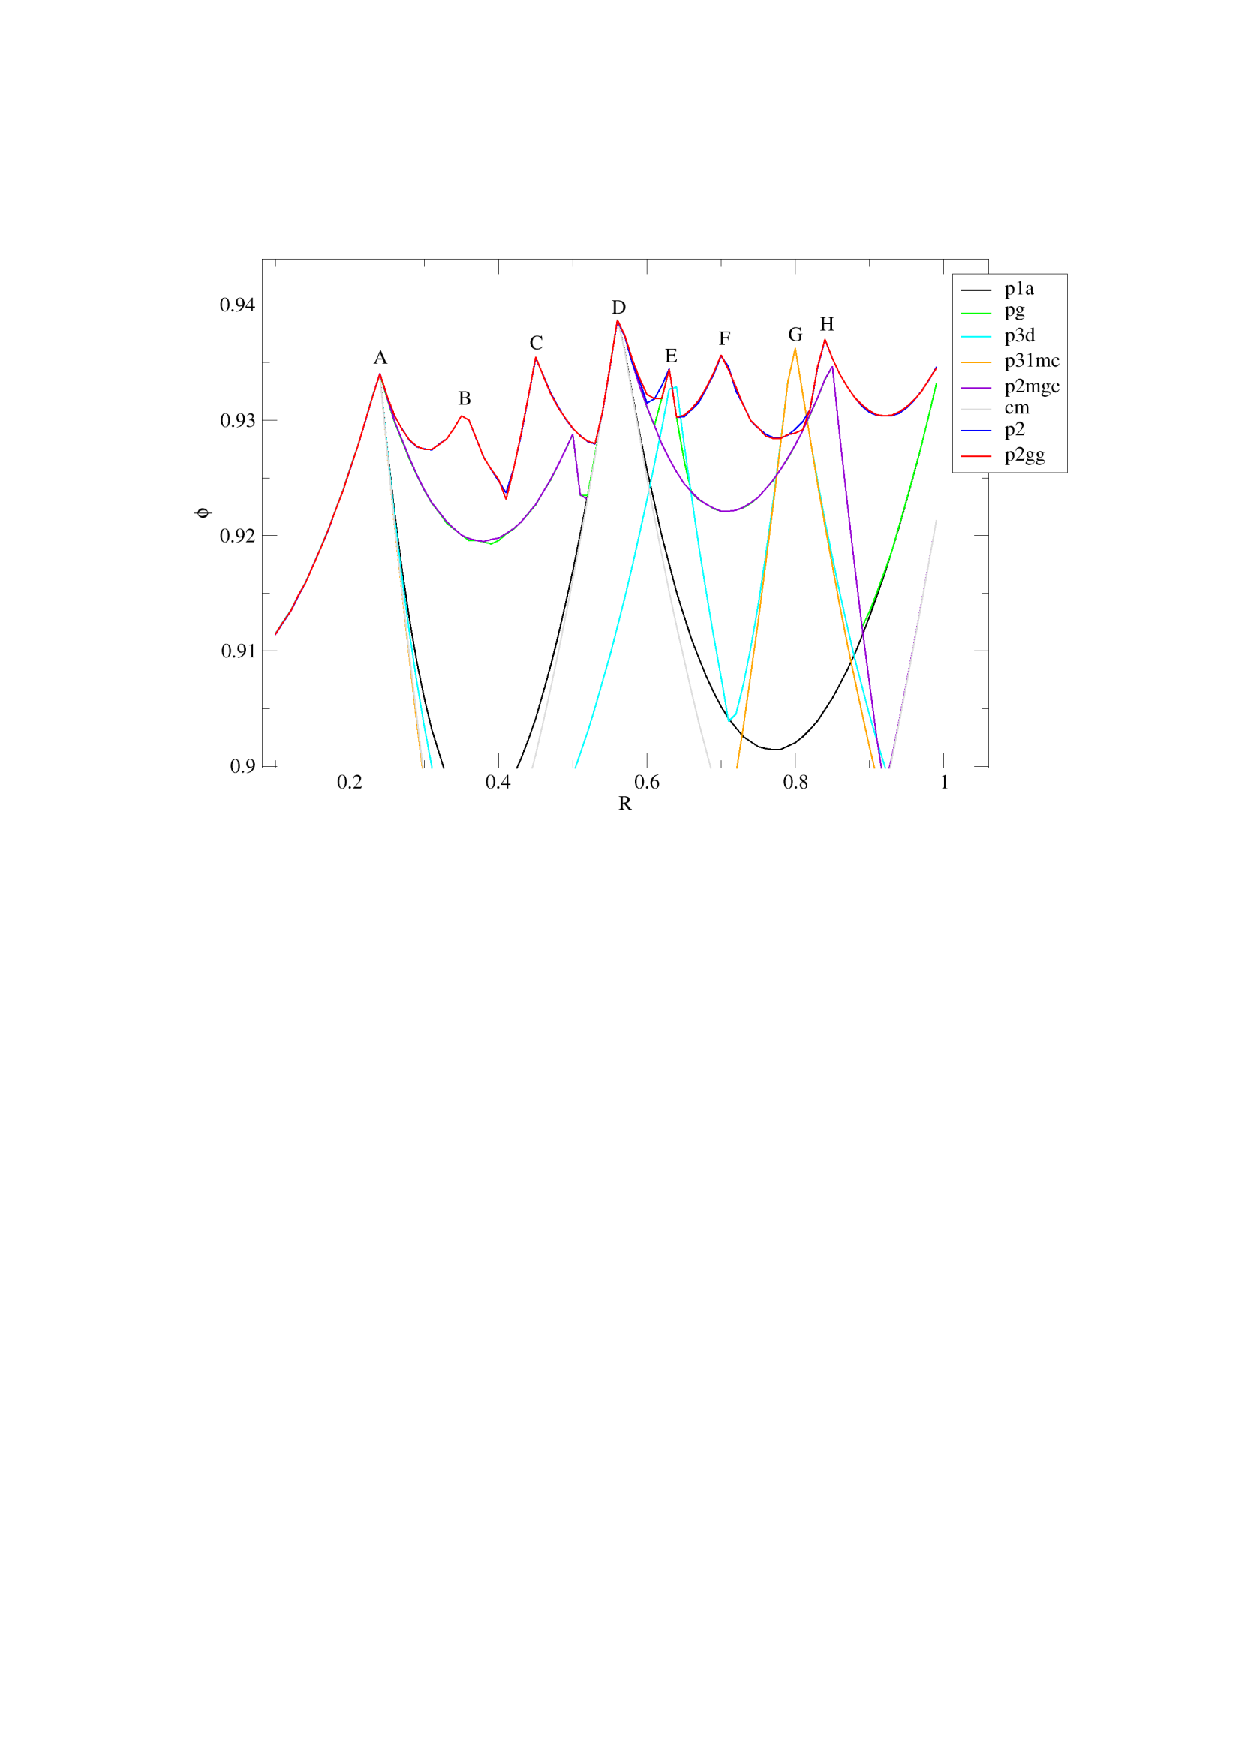
\includegraphics[width=\textwidth]{crystal-packing-dist}
    \caption{The packing fraction of Snowmen as a function of radius for $d=1$}
    \label{fig:crystal packing dist}
\end{figure}


\section{Packing Trimers}

The packing of trimers

\towrite{How trimers pack}

\towrite{Comparing to crystals}

\begin{figure}
    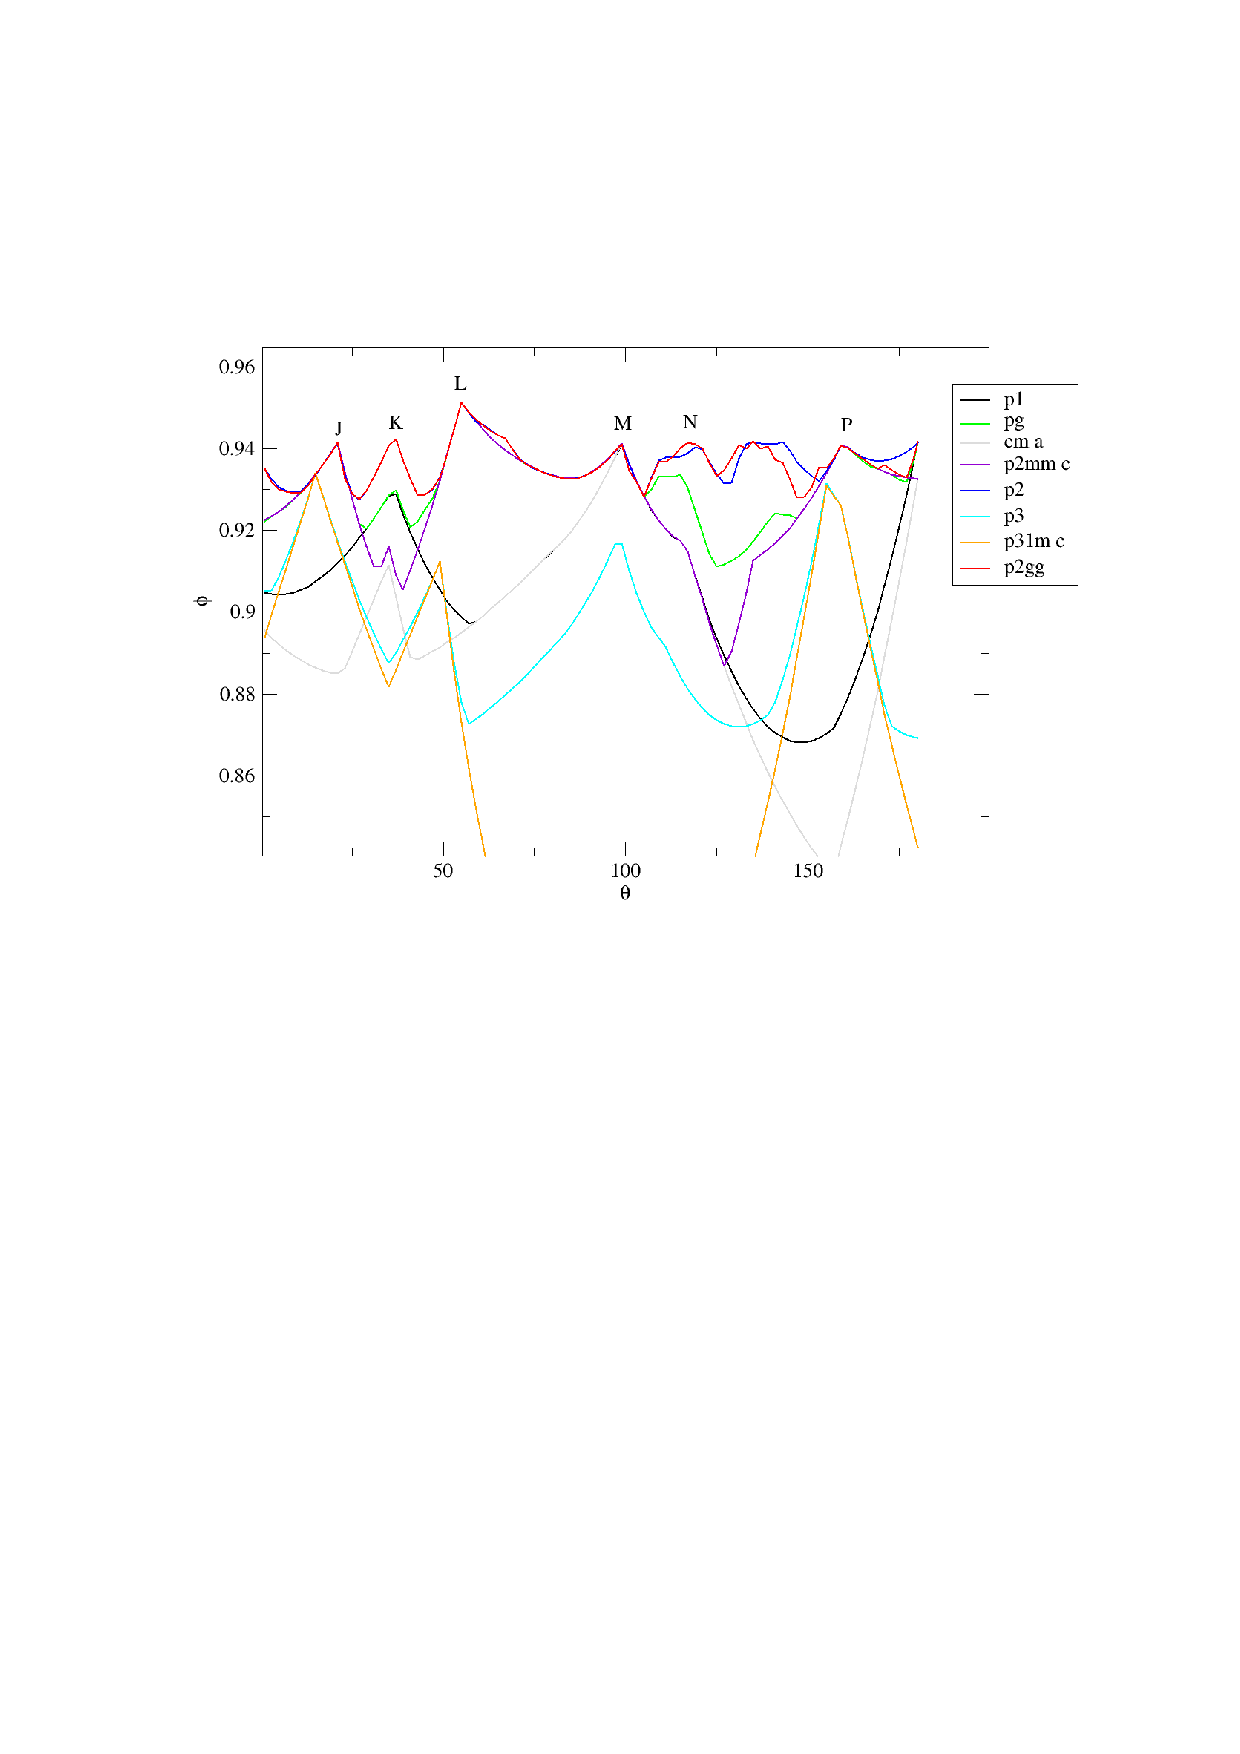
\includegraphics[width=\textwidth]{crystal-packing-theta}
    \caption{The packing fraction of Trimers as a function of theta with $r=0.7$ and $d=1$}
    \label{fig:crystal packing theta}
\end{figure}

\section{Low Temperature Packings}

As a way of detecting molecules that are slow to crystallise the random packings were cooled relatively quickly to a low temperature, at which point they were then equilibrated and the inherent structure found. These packings were significantly different to the high temperature ones, with the densest packing achieving a packing fraction of 1.05\tocheck~\figref{radius-low}. This does illustrate one of the problems using packing fraction for the analysis of soft discs, their overlap allows much greater packing fractions.


\begin{figure}
    \centering
    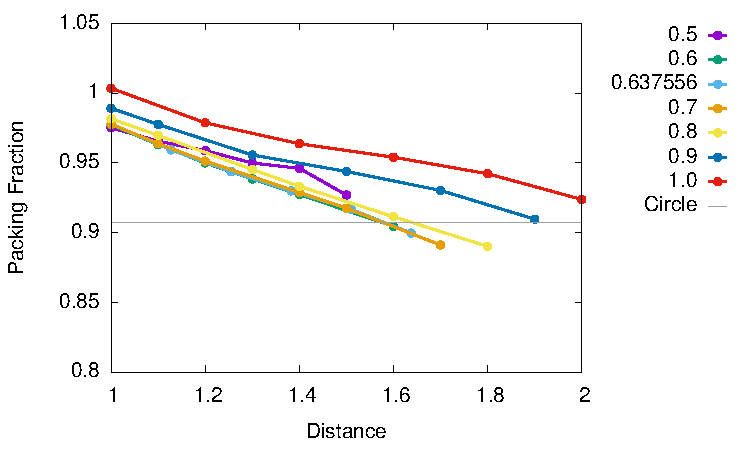
\includegraphics[width=0.75\textwidth]{dist-low}
    \caption[Packing fraction of snowmen as a function of distance ($T=0.4$)]{The packing fraction as a function of distance for the snowman molecules. The system was equilibrated at $T=0.4$ before quenching to the inherent structure. For reference the optimal circle packing of 0.91 is included.}
    \label{fig:snowman dist low}
\end{figure}

\begin{figure}
    \centering
    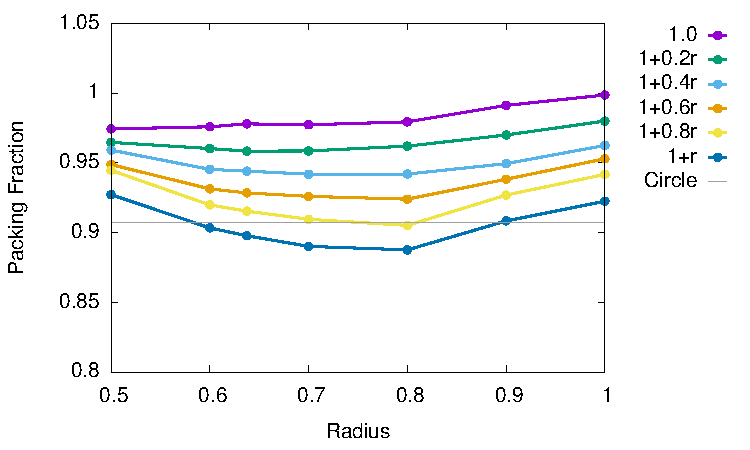
\includegraphics[width=0.75\textwidth]{radius-low}
    \caption[Packing fraction of snowmen as a function of radius ($T=0.4$)]{The packing fraction as a function of radius for the snowman molecules. The system was equilibrated at $T=0.4$ before quenching to the inherent structure. For reference the optimal circle packing of 0.91 is included.}
    \label{fig:snowman radius low}
\end{figure}

\section{Choosing Interesting Shapes}

All of the shapes that we have seen are interesting, the characteristics they display are diverse and result in pretty figures. For this project we are interested in molecules resistant to crystallisation that have a diverse range of properties. One molecule that stands out is the Snowman $r=0.637556,\,d=1.637556$, we know this molecule has a compact packing which should allow it to form a high-entropy low-enthalpy crystal packing, yet there is no ordering past the shell of nearest neighbours. This lack of crystal formation implies that the molecule is a good glass former and studying the properties could reveal what is preventing it from crystallising.

Having chosen the Snowman $r=0.637556,\, d=1.637556$ molecule as a candidate for further study the Snowman $r=0.637556,\,d=1.0$ and Trimer $r=0.637556,\,d=1.0,\theta=120$ were chosen. The primary focus of this thesis is on the effect of shape on the properties of a molecule. By keeping the radius ratio the same we are keeping the focus on the arrangement on the particles in space. The $r=0.637556\,d=1.0$ Snowman was chosen for being similar to the $r=0.7,\,d=1.0$ Snowman which showed strong short range ordering. The Trimer was chosen for having a large concavity between the two small molecules, the concavity is larger than any of the molecules and it is interesting to see how this affects the properties.



